\chapter{Métodos de Control del Huanglongbing en México}

En este capítulo, se describen las normas y los mecanismos institucionales para el tratamiento del HLB en México, así como el protocolo que se instruye seguir a los agricultores ante la detección de un árbol con evidentes síntomas de la enfermedad, además, se muestran los métodos empleados cuando existe sospecha de un brote. Este capítulo da fundamento a la forma en la que se han simulado el campo y los métodos de control aplicados en él en este trabajo, puesto que, como se verá más adelante en el siguiente capítulo, el objetivo principal de este experimento es poner a prueba las medidas en el combate y prevención de las infecciones por esta enfermedad en México. El Capítulo analiza los manuales y protocolos publicados por la autoridad correspondiente, con la idea de tener información oficial de la forma en la que se trata a esta enfermedad en el país, y de este modo tener una simulación congruente.\\
En México, en el año en el que se escribe esta tesis, es atribución de la Secretaría de Agricultura y Desarrollo Rural (SADER), llamada en sexenios pasados Secretaría de Agricultura, Ganadería, Desarrollo Rural, Pesca y Alimentación (SAGARPA), el establecimiento de las medidas fitosanitarias pertinentes en virtud de la  prevención y el control de las plagas capaces de potencialmente mermar las cosechas de vegetales, así como sus productos y subproductos. Es importante puntualizar que los productos \textit{fitosanitarios} son, en general, aquellas sustancias capaces de prevenir o combatir a las plagas, que para el caso que ocupa a este trabajo, suelen ser los insecticidas usados para combatir al vector transmisor \textit{Diaphorina citri}, o en un caso más remoto; bactericidas o antibióticos para atacar directamente a la bacteria que causa la enfermedad. Además, existe un organismo descentralizado de la SADER, el SENASICA, cuyo fin es el de proteger los recursos agrícolas de plagas y enfermedades de cuarentena. Además, se encarga de la regulación y el fomento de los sistemas de reducción de riesgos de contaminación de alimentos, para dar certeza a los productos vegetales y animales, así como sus derivados, para el comercio nacional e internacional.\cite{cortez2010control}

\section{La Campaña contra el Huanglongbing de los Cítricos}

Dado que el SENASICA es el responsable de implementar las acciones encaminadas a la prevención, control y erradicación de las plagas en el territorio nacional, particularmente para el caso del Huanglongbing, se han tomado algunas medidas fitosanitarias como: vigilancia epidemiológica en huertos comerciales y zonas urbanas, así como el control químico y biológico del vector, tanto en jardines como en huertos comerciales de zonas en las que existe concurrencia de focos de infección. Este conjunto de acciones constituyen a la Campaña contra el Huanglongbing de los Cítricos. Las zonas a las que se dirige esta campaña, son denominadas \textit{ARCOs}. El sentido de los ARCOs es el de agrupar todas las actividades de vigilancia, control biológico y control químico en un área estratégicamente definida en extensión y forma, en virtud de reducir la posibilidad de que los focos de la epidemia alcancen mayores proporciones, y es en este contexto que es de interés revisar la metodología usada por esta campaña para la detección del Huanglongbing, así como las acciones a realizar ante la detección de esta enfermedad, tanto en las plantas como en los psílidos infectivos que habiten en huertas comerciales y zonas urbanas. Finalmente, esta sección busca puntualizar los criterios para la búsqueda y control de los árboles infecciosos.

\subsection{Búsqueda y detección del Huanglongbing}
A lo largo del país, a través de los huertos comerciales y domésticos, tanto en las plantas de cítricos como en algunas ornamentales, existen dos formas de detectar el HLB. La primera es indirecta, mediante la colecta de los insectos transmisores que son posteriormente analizados para detectar a la bacteria causante. En la forma directa, se da la búsqueda de síntomas de primera mano en la materia vegetal.\\ El proceso en los huertos comerciales de las zonas citrícolas que no tienen presencia de la enfermedad, es homogéneo, sin embargo, el muestreo en los huertos es priorizado dependiendo de algunas condiciones que los hagan más propensos a contraer la enfermedad. Los criterios son varios, como que en los huertos existan plantas que tengan menos de 10 años de edad, que se localicen junto a lagunas u otros cuerpos de agua, o que la huerta sea joven y esté próxima a una adulta; otras condiciones para priorizar una huerta son: que se localice cerca de una frontera, costa, área urbana o algún centro donde se concentren cítricos, que colinde con estados o zonas con presencia de HLB o incluso las carreteras que conducen a ellos.\\
El primer paso para la detección indirecta es la toma de una muestra, en cada huerto, de cierta cantidad de psílidos adultos. La muestra se hace manualmente, por lo general con una aspiradora o algún otro instrumento que asegure a los insectos, que posteriormente son colocados en viales con alcohol etílico y son etiquetados. Una vez colectadas las muestras, éstas son enviadas al laboratorio con la menor demora posible, para de estar en condiciones de detectar oportunamente cualquier caso positivo y con ello encontrar los posibles focos de infección. El personal que toma las muestras se auxilia de un teléfono en el que registra la geolocalización de dichas muestras.\\
La minoría de los huertos en los que se colectan las muestras son mayores a cinco hectáreas, habiendo incluso entidades en las que, debido a que los huertos son pequeños, las muestras son en su totalidad en huertos menores a cinco hectáreas. Si el huerto es menor a cinco hectáreas, el muestreo es metódico, y se colectan entre 5 y 10 insectos de cada planta. En total se eligen veinticuatro plantas de la siguiente forma: supongamos que el huerto tiene forma de cuadrilátero y se elige una cara de éste, preferentemente la que recibe predominantemente el soplar del viento la mayor parte del tiempo, en el borde de esta cara se elige el árbol que esté en alguna de las dos esquinas, luego se dejan tres árboles a lo largo de este borde y se vuelve a muestrear, de modo como se ve en la figura 3.1. Una vez trazado el primer patrón, se toman los dos árboles que estén en la parte media de la línea de muestreo, y desde ellos se sigue con el mismo procedimiento, pero esta vez con dirección al centro del huerto, lo que resulta en un patrón en toda la arista del cuadrado en el que hay un muestreo cada tres árboles, a esto se le llama método en «T».

\begin{figure}[H]
\centering
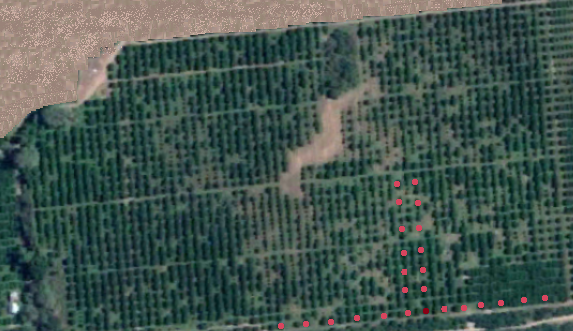
\includegraphics[width=0.6\textwidth,keepaspectratio=true]{images/C3/T.png}
\caption{Ilustración del método en «T». Una huerta cuyos árboles examinados se marcan en rojo.}
\end{figure}

Cuando los huertos son mayores a cinco hectáreas el método es muy parecido, salvo por el hecho de que en este caso se emplea dos veces el procedimiento descrito anteriormente, aplicando el segundo en la cara opuesta a la cara en la que se aplicó el anterior, esto se puede observar en la figura 3.2.

\begin{figure}[H]
\centering
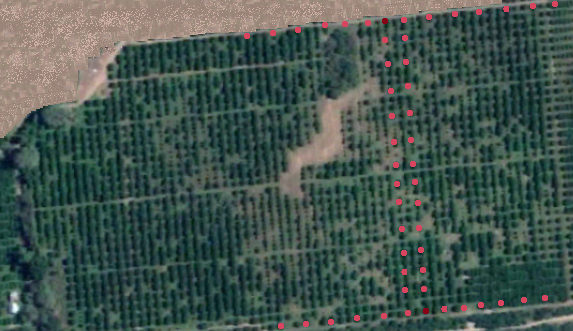
\includegraphics[width=0.6\textwidth,keepaspectratio=true]{images/C3/T2.png}
\caption{Ilustración del método en doble «T».}
\end{figure}

En las zonas urbanas existen rutas de muestreo que se recorren mensualmente, las zonas que recorren estas rutas están constituidas por una media de tres poblaciones o comunidades en las que no existe presencia de la enfermedad pero sí del psílido, se pone especial interés en los árboles de limón mexicano y se toma una muestra por cada comunidad, pudiendo contener hasta cien individuos, y tomando muestras de cinco árboles distintos en los períodos de alta infestación. Los lugares de recolección son camellones, jardineras o parques. 

\subsection{Protocolo ante la detección de muestras positivas a Candidatus Liberibacter}
Ante la detección de casos positivos en las muestras tomadas durante los procedimientos descritos anteriormente, ya sea a través de las muestras de psílidos adultos o en las del material vegetal con síntomas (que se detallan e ilustran en el capítulo anterior: Conceptos Preliminares), existen diferentes medidas a tomar, dependiendo del caso de la detección, pero más allá de qué medidas se implementen, se debe tener presente que es la Dirección General de Sanidad Vegetal la autoridad encargada de gestionar las acciones procedentes.\\

%4.1
Cuando se detectan psílidos infectivos en huertos comerciales, después de algunos procedimientos institucionales en los que no se profundizará, se designa a un responsable, miembro de algún organismo gubernamental, para que coordine las acciones a llevar a cabo para hacer frente a la amenaza. Estas actividades incluyen colectar psílidos o directamente comenzar con su control, y de ser necesario, la búsqueda de síntomas en el área de influencia de la detección, y posterior a esto se rinde un informe en un plazo no mayor a diez días hábiles a partir de la conclusión de estas actividades.\\
La exploración para la detección de síntomas en los cítricos comienza con la revisión de la totalidad de los árboles que conforman el huerto en el que se ha detectado el brote; es importante enfatizar que esta revisión se limita a buscar síntomas, algo que contribuye a combatir el brote pero no da una certeza total, dado que, como se ha dicho antes, algunos árboles muestran sus síntomas mucho tiempo después de ser portadores. Si se encuentran síntomas en un árbol, se colectan algunas piezas de material vegetal y se analizan, y en caso de que se confirme un resultado positivo, se instruye al productor realizar una aplicación de insecticida contra el vector. Además, se \textit{delimita el brote} y se promueven las \textit{actividades para su manejo}, dos temas que se tratarán más adelante. Si los resultados obtenidos después de estas acciones no son los deseables, la huerta es considerada como un «punto rojo» para muestreo y diagnóstico, por lo que se instruye nuevamente al productor aplicar insecticida contra el vector.\\
El muestreo de psílidos se hace mediante la colecta de ellos de forma simultánea a la búsqueda de síntomas, descrita anteriormente. La forma de recabar a estos ejemplares es parecida a la descrita anteriormente, se toman veinte plantas, esta vez dejando dos árboles entre cada árbol elegido, en lugar de tres como en el caso anterior, pero manteniendo la misma estructura perpendicular y colectando también de cinco a diez insectos por árbol. Si hay alguna localidad urbana a menos de un kilómetro de la huerta donde se detectó la muestra positiva, existe una alta probabilidad de encontrar HLB en ella, de modo que esta también debe ser analizada. Si alguna huerta reincide en tener psílidos infectivos, la autoridad competente notifica al productor la responsabilidad del control del psílido.\\
\begin{figure}[H]
\centering
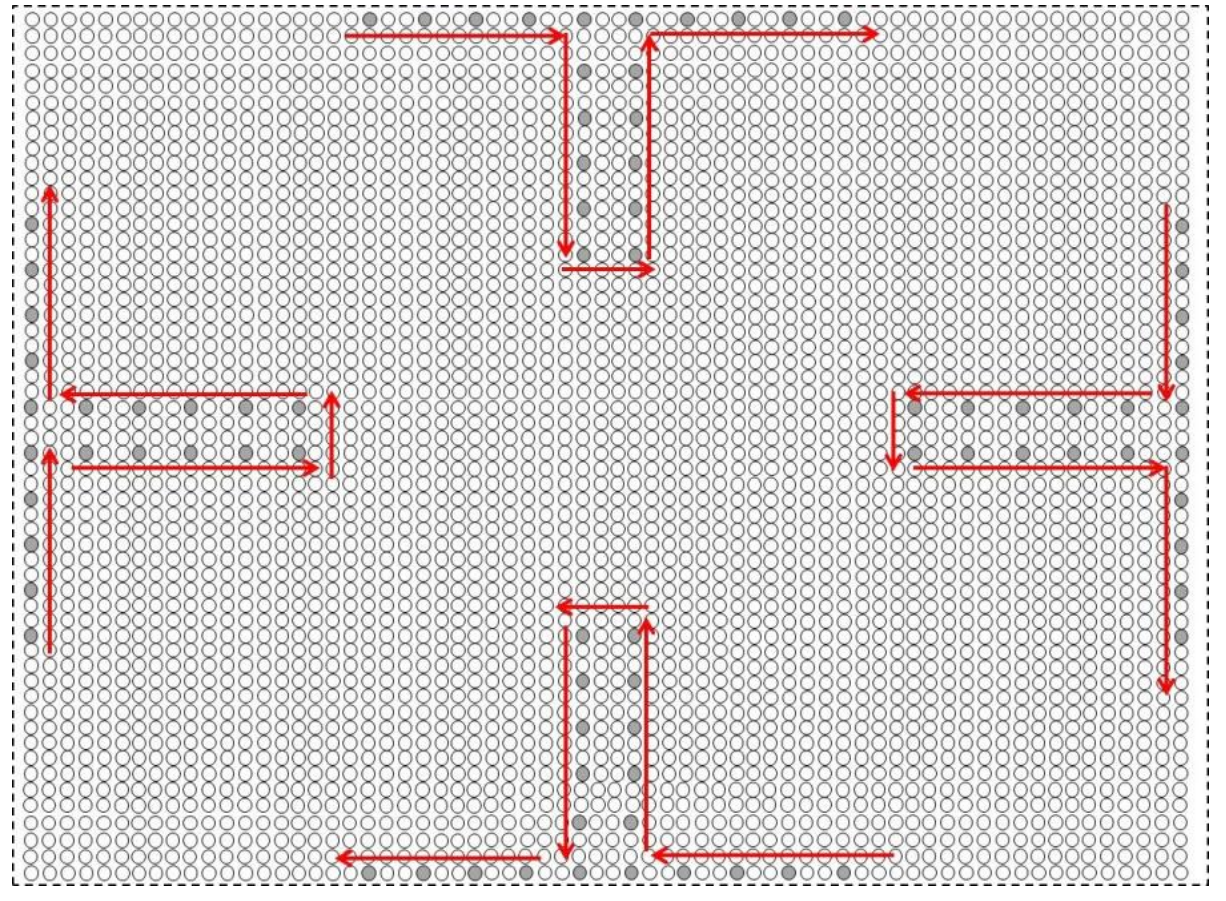
\includegraphics[width=0.8\textwidth,keepaspectratio=true]{images/Norm/MT.png}
\caption{Ilustración del método en T. Manual operativo de la Campaña contra el Huanglongbing de los Cítrico}
\end{figure}
%4.2
Cuando se detectan psílidos infectivos en rutas de muestreo de zonas urbanas, se revisa la totalidad de las plantas de la localidad donde se detectó la infección y se toman muestras de materia vegetal de las plantas que presenten la sintomatología característica del HLB y paralelamente se capturan algunos psílidos por cada manzana de casas. Si las pruebas resultan positivas, la autoridad aplica insecticida en toda la manzana y en las colindantes. Si los resultados son negativos, solamente se aplica insecticida puntualmente en las plantas con psílidos positivos.\\
%4.3
Respecto a la delimitación de los brotes de HLB, existen tres ámbitos, en primer lugar, naturalmente se empieza con la formación de brigadas para su posterior movilización, y entonces se implementan las acciones para delimitar el foco inicial en los sitios con detecciones, esto a un nivel local, y para un nivel regional se emprenden las acciones encaminadas a delimitar los focos en toda la comarca. La formación y movilización de las brigadas comienza con la notificación oficial  de la confirmación de HLB, y la autoridad competente pone en marcha a los equipos con los insumos necesarios que llevarán a cabo las acciones, estas brigadas contarán con técnicos para reconocer los síntomas de HLB y los instrumentos necesarios para el registro de la localización de las plantas sospechosas\\
En el segundo ámbito, en el encaminado a delimitar el foco inicial de los sitios con detecciones, se realiza una exploración intensiva en el huerto donde se detectó el cítrico positivo, siguiendo la figura 3.4:\\

\begin{figure}[H]
\centering
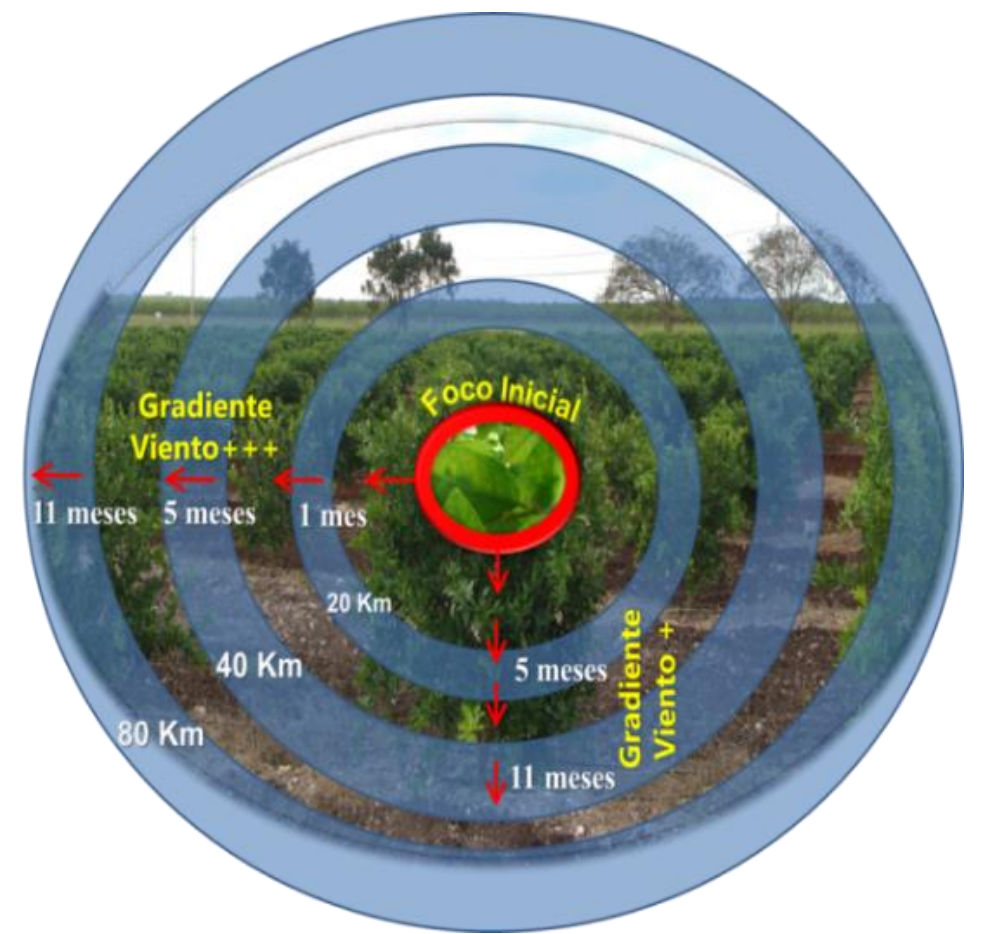
\includegraphics[width=0.5\textwidth,keepaspectratio=true]{images/Norm/figura 7-10.png}
\caption{Delimitación del foco inicial. Manual operativo de la Campaña contra el Huanglongbing de los Cítrico}
\end{figure}

En un siguiente nivel en escala, las acciones para determinar los focos regionales están condicionadas por las direcciones de los vientos dominantes, que favorecen la dispersión del HLB a nivel regional. La delimitación de estos focos de infección se hace mediante recorridos en rutas de muestro que se trazan a partir de la detección de una planta positiva en muestreos cada veinte kilómetros.

%4.4, 4.5
Finalmente, la divulgación y el manejo del brote son de suma importancia y son responsabilidad de la autoridad, esta divulgación debe hacerse oportunamente entre los productores, organizaciones relacionadas con la producción y las organizaciones nacionales de otros países a través de la Organización Norteamericana de Protección a las Plantas (NAPPO). Para manejar los brotes de HLB, en principio, habría de bastar con la localización y eliminación de las plantas enfermas, el control regional y de los focos de infestación del psílido, además del uso de plantas producidas en viveros certificados. En las zonas que padecen una alta incidencia de HLB, se implementan programas intensivos de nutrición para alargar la vida útil de los huertos afectados.

\subsection{Control del psílido asiático de los cítricos a través de ARCOs}

Como se ha dicho antes, el control regional del psílido se hace de forma coordinada con los productores en zonas citrícolas delimitadas estratégicamente en bloques mayores a mil hectáreas, esto se hace en algunas épocas durante lapsos cortos mediante la rotación de insecticidas con distintos grupos toxicológicos, y, de ser posible, agentes de control biológico. Estas zonas son llamadas Áreas Regionales de Control, a partir de ahora, «ARCOs».  Por otro lado, los focos de infestación son controlados a través del monitoreo quincenal por parte de los productores de forma conjunta. Lo anterior se debe a que ambos tipos de control, el regional y el de focos, son necesarios en virtud de la alta capacidad de dispersión del psílido a distancias largas, su constante migración entre los huertos y plantas, y la dificultad para evitar que infecten las plantas en las que se alojan. Los ARCOs son definidos cada año con base en los datos epidemiológicos, contemplando la organización, el monitoreo, el control químico, y el control biológico.
%Monitoreo del psílido
Con el objetivo de conocer los patrones en el comportamiento del vector en las zonas de los ARCOs, en las regiones, y finalmente en el país, el  psílido es monitoreado. Esta práctica, además, contribuye en la identificación de los brotes de este insecto en algunas zonas citrícolas en las que se pretenda controlar los focos de infestación. Para lograr esto, se monitorea al insecto en las huertas que tengan por lo menos 2.5 hectáreas, preferentemente aledañas a cuerpos de agua, carreteras o caminos, y que tengan una distancia entre ellas de aproximadamente 700 metros. La captura se hace mediante trampas de plástico con pegamento que se colocan en los árboles (Figura 3.5), estas trampas son esencialmente una placa amarilla cuadriculada en la que los insectos se quedan pegados al contacto, la cuadrícula tiene cinco por siete cuadrados de 2.5 centímetros para facilitar el conteo de los insectos atrapados en ella. Las trampas se localizan en las plantas de las orillas de los huertos, dispuestas en grupos de veinte y dejando un árbol libre entre cada dos árboles con trampa, en la última o penúltima fila o columna de árboles. A continuación (Figura 3.6), se ilustra la disposición de las trampas, incluso si el huerto no está dispuesto en forma de cuadrícula.

\begin{figure}[H]
\centering
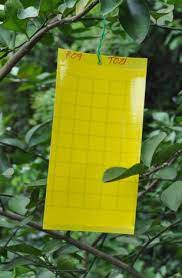
\includegraphics[width=0.3\textwidth,keepaspectratio=true]{images/C3/Trampa.jpg}
\caption{Trampa de plástico con pegamento colocada en un árbol. Imagen extraída de documentación oficial de SAGARPA}
\end{figure}


\begin{figure}[H]
\centering
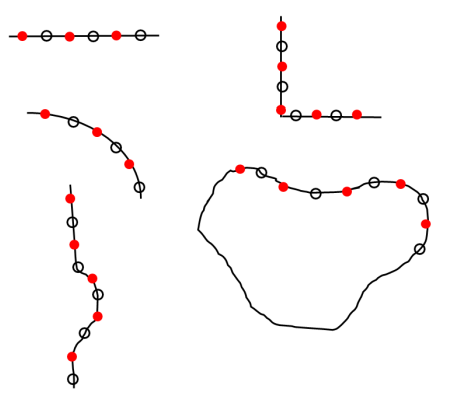
\includegraphics[width=0.5\textwidth,keepaspectratio=true]{images/Norm/ar.png}
\caption{Ejemplo de disposición de trampas en huertos irregulares. Manual operativo de la Campaña contra el Huanglongbing de los Cítrico}
\end{figure}

La distancia entre los grupos de trampas no puede superar los 700 metros, de tal forma que se cubra la totalidad de la superficie del ARCO, procurando que sus localizaciones sean equidistantes. Luego de que una trampa se coloca y el adhesivo queda expuesto, tiene una vida útil de catorce días, pues es luego de dos semanas que se retira para su monitoreo y cambio. En cada revisión, se cuentan los adultos del psílido y los datos son capturados a través del Sistema de Monitoreo de Diaphorina (SIMDIA). \textit{http://www.siafeson.com/simdia.php}.\\

\section{Métodos de control de las Campañas Mexicanas contra el HLB}

A continuación, se describen de forma particular los métodos de control usados oficialmente en las Campañas contra el HLB.

\subsection{Control Biológico en ARCOs}%IX
Existe otro tipo de control del psílido asiático de los cítricos, el control biológico, que tiene buenas implicaciones en lo que a cuidado del medio ambiente se refiere, teniendo grandes resultados en la reducción de la población de estos insectos. Las estrategias de control biológicas son utilizadas en los ARCOs conjuntamente con las sintéticas, estas estrategias son, por lo común, parasitoides y hongos entomopatógenos.\\
En las áreas especiales, como huertas abandonadas o zonas urbanas que se encuentren dentro o aledañas al control de los ARCOs, se emplea la liberación estratégica de algunos parasitoides, como Tamarixia radiata, debido a que existen algunas limitantes para el empleo de insecticidas, como riesgos de salud pública o desinterés. Las dosis que se liberan de estos parasitoides son de 100, cada 20, 50 o 100 metros, en función del grado de infestación. Existen otras estrategias, como la utilización de depredadores, por ejemplo, varias especies de Chrysoperla, o el uso de hongos entopatógenos, que causan enfermedad en el psílido, como Isaria fumosorosea o Metarhizium anisopliae, que en el laboratorio tienen niveles de mortalidad del 93.01\% de las ninfas y el 95.22\% en adultos, y en el campo mexicano reducen las poblaciones entre 48\% y 90\%.

\subsection{Eliminación de plantas}%XI

La indicación del protocolo establece que debe haber al menos cuatro monitoreos por año en los que se revise la totalidad de las plantas de cada huerta, con el fin de detectar oportunamente el HLB. Deben eliminarse de inmediato las plantas que presenten síntomas de la enfermedad cuando esta esté muy dispersa. Los recorridos para encontrar plantas con síntomas son realizados por personal capacitado, quienes marcan a las que tengan síntomas con listones, y en las plantaciones en las que la disposición sea en hileras, se marcan también las dos plantas de la hilera, que son vecinas al árbol sintomático. Posteriormente, el árbol es revisado por un técnico especializado y en caso de que el diagnóstico sea ratificado, según el protocolo: \textit{Cuando el HLB se encuentra muy disperso en el área, no se considera necesario que estas plantas sean muestreadas para proceder con la eliminación.} La poda no funciona para el control del HLB, es necesario cortar la planta y aplicar herbicida al tocón. No es necesario incinerar la planta cortada, pero sí se ha de evitar la replantación hasta que no disminuyan las poblaciones del insecto, ya que las plantas nuevas son más susceptibles, también se ha de prestar atención a los niveles de la enfermedad, puesto que no es recomendable la replantación si ésta se encuentra por encima del 5 \%.\\
En los traspatios, la responsabilidad es de los organismos auxiliares de sanidad vegetal, en contraste con lo que sucede con las huertas, en las que la responsabilidad es de los productores, quienes además promueven que no se establezcan cítricos y otros hospedantes del HLB en zonas urbanas. Lo anterior se suma a la exigencia de programas de certificación de material propagativo de cítricos, de tal forma que los viveros cuenten con mallas que impidan el paso del psílido asiático de los cítricos.


\subsection{Control Regional en huertas convencionales y huertas orgánicas}%VII
El territorio mexicano es diverso en condiciones agroecológicas y por esta razón tiene diversos escenarios epidemiológicos en lo que al HLB respecta, de modo que el control regional no es homogéneo. No obstante, el control regional se realiza en todos los casos mediante la aplicación de insecticidas, algunos foliares, que están dirigidos a los psílidos adultos pero también suprimen unos cuantos huevecillos o ninfas, además de minimizar el daño a insectos benéficos y prevenir el surgimiento de poblaciones en primavera si se aplica en invierno; por otro lado, están los insecticidas sistémicos al suelo, especialmente en plantas jóvenes como medida profiláctica. También es posible aplicar insecticida de forma extraordinaria en los focos de infección, una vez se tenga la certeza de que lo son, mediante las trampas de las que se ha hablado anteriormente en este texto. Lo deseable es que la aplicación sea en toda la región, pero si esto no es posible, la prioridad es la periferia.\\
El psílido asiático de los cítricos no es la única plaga que aqueja a los cultivos, de modo que se ha de corroborar la compatibilidad de los insecticidas, ya que algunos, como el aceite mineral, no deben mezclarse con azufre. Las aplicaciones han de ser totales, preferentemente, ya que, además de evitar contribuir al desarrollo de resistencia, también se combaten otras plagas como  el minador de los cítricos, la araña roja, o el ácaro blanco. El control regional en huertas orgánicas es especialmente importante, debido a la gran cantidad de huertos de producción orgánica y  este tipo de huerto representa un desafío especial, de modo que es necesario un plan más sólido para la zonas de producción que contengan esta mayoría de huertos. Los pulguicidas orgánicos no son eficaces en el manejo de grandes cantidades de psílidos, de modo que cuando existe un contagio mayor, es imprescindible el uso de pulguicidas convencionales, lo que hace que el huerto orgánico pierda tal calidad.

